\documentclass[../../main.tex]{subfiles}

\graphicspath{{../../image/}{../../figure/}}

\begin{document}

\section{概率潜变量}\label{section:ch16-概率潜变量}

我们在\cref{section:ch16-主成分分析}中已经看到 PCA 可以定义为数据在低维子空间上的线性投影，这个低维子空间的维度比原始数据空间的维度小。每个数据点被映射到由\eqref{align:ch16-z最优}定义的唯一的量 $z_{ni}$，我们可以将这些量视为确定性的潜变量。为了引入和论证连续概率潜变量，本节会展示，PCA 也可以表示为概率潜变量模型的最大似然解。这种 PCA 的重新表述，称为概率 PCA，与传统 PCA 相比，有如下优势。
\begin{itemize}
  \item 概率 PCA 模型表示了 Gauss 分布的一种约束形式，在仍然能够捕捉数据集中主要相关性的同时，还可以限制自由参数的数量。
  \item 我们可以为 PCA 推导出一种 EM 算法，该算法在只需要少数几个主特征向量的情况下计算效率很高，而且能避免将计算数据协方差矩阵作为中间步骤进行计算（见\cref{subsection:ch16-PCA的EM算法}）。
  \item 概率 PCA 模型与 EM 算法的结合使我们能够处理数据集中缺失的值。
  \item 可以原则性地构造概率 PCA 模型的混合模型并使用 EM 算法进行训练。
  \item 似然函数的存在使得我们可以与其他概率密度模型直接进行比较。相比之下，传统 PCA 模型会给予靠近主成分子空间（也可简称主子空间）且距离训练数据任意远的数据点一个较低的重建成本。
  \item 概率 PCA 可用于建模类-条件密度，因此可应用于分类问题。
  \item 概率 PCA 模型可以生成性地运行以提供来自分布的样本。
  \item 概率 PCA 构成了基于 Bayes 方法处理 PCA 的基础，我们可以从数据中自动找到主成分子空间的维度（Bishop, 2006）。
\end{itemize}

将 PCA 作为概率模型的这种表述是由 Tipping and Bishop (1997; 1999) 以及 Roweis (1998) 独立提出的。正如我们稍后将看到的，它与因子分析（factor analysis）（Basilevsky, 1994）密切相关。

\subsection{生成式模型}\label{subsection:ch16-生成式模型}

概率 PCA 是线性-Gauss 框架的一个简单例子，其中所有的边缘分布和条件分布都是 Gauss 分布。我们可以首先通过引入对应于主成分子空间的、明确的 $M$ 维潜变量 $\bm{z}$ 来构建概率 PCA。接下来，我们定义一个关于潜变量的 Gauss 先验分布 $p(\bm{z})$，以及基于潜变量值的、$D$ 维观测变量 $\bm{x}$ 的 Gauss 条件分布 $p(\bm{x}|\bm{z})$。具体来说，关于 $\bm{z}$ 的先验分布由零均值、单位协方差的Gauss分布给出：
\begin{align}
  p(\bm{z})=\mathcal{N}(\bm{z}|\bm{0},\bm{I}).
  \label{align:ch16-先验}
\end{align}

同样，观测变量 $\bm{x}$ 的条件分布，基于潜变量 $\bm{z}$ 的值，也符合 Gauss 分布：
\begin{align}
  p(\bm{x}|\bm{z})=\mathcal{N}(\bm{x}|\bm{W}\bm{z}+\bm{\mu},\sigma^2\bm{I}).
  \label{align:ch16-条件分布}
\end{align}

把上述模型的形式正式表述如下。

\begin{definition}[概率 PCA]\label{definition:ch16-概率PCA}
设 $\bm{z}$ 是 $M$ 维连续潜变量，$\bm{x}$ 是 $D$ 维观测变量。若它们的联合分布由
\begin{align*}
  p(\bm{z})=\mathcal{N}(\bm{z}|\bm{0},\bm{I}),\qquad
  p(\bm{x}|\bm{z})=\mathcal{N}(\bm{x}|\bm{W}\bm{z}+\bm{\mu},\sigma^2\bm{I})
\end{align*}
给出，其中 $\bm{W}$ 是 $D\times M$ 矩阵、$\bm{\mu}$ 是 $D$ 维向量、$\sigma^2>0$ 是控制条件分布方差的标量，则称 $(\bm{x},\bm{z})$ 服从概率 PCA（probabilistic PCA, PPCA）模型，称 $\bm{W}$ 的列所跨越的数据空间中的线性子空间为该模型的子空间。
\end{definition}

% SUPPLEMENT: parent=definition:ch16-概率PCA; kind=motivation; location=紧随其后的 remark（重构新增）
\begin{remark}（重构新增）
概率 PCA 的动机是给\cref{section:ch16-主成分分析}中纯代数的 PCA 补上一个概率生成机制，从而可以用最大似然而不是“方差最大”这类几何准则来确定参数。生成图像的过程可以这样读：先从 $\mathcal{N}(\bm{0},\bm{I})$ 抽取一个低维码字 $\bm{z}$，用 $\bm{W}$ 把它线性地搬到 $D$ 维空间中，再加上均值为 $\bm{\mu}$ 的位置偏移，最后叠加各向同性的 Gauss 噪声 $\mathcal{N}(\bm{0},\sigma^2\bm{I})$。因此 $\bm{W}$ 的列张成的正是数据的“理想”低维子空间，而 $\sigma^2$ 度量数据偏离该子空间的程度。

条件的含义需要逐条说明。第一，$\bm{z}$ 的先验取零均值、单位协方差，这不是实质限制：若先验是 $\mathcal{N}(\bm{m},\bm{\Sigma})$，重新定义 $\bm{W}'=\bm{W}\bm{L}$、$\bm{\mu}'=\bm{\mu}+\bm{W}\bm{m}$（其中 $\bm{L}\bm{L}^{\mathsf T}=\bm{\Sigma}$）即可把模型化为本定义的形式，观测分布完全不变（见\cref{exercise:ch16-04}）。第二，条件协方差取 $\sigma^2\bm{I}$ 而不是一般的正定矩阵，正是概率 PCA 区别于因子分析的地方，它使 $\bm{x}$ 的各分量在给定 $\bm{z}$ 时条件独立，并且使模型对潜空间的旋转不变（见\cref{proposition:ch16-旋转不可识别}）。第三，要求 $\sigma^2>0$：若 $\sigma^2=0$，$\bm{x}$ 将以概率 $1$ 落在 $\bm{W}$ 的列空间这个零测集上，边缘密度退化而不再有密度，最大似然问题也没有意义。
\end{remark}

其中 $\bm{x}$ 的均值是 $\bm{z}$ 的一般线性函数，受 $D\times M$ 维矩阵 $\bm{W}$ 和 $D$ 维向量 $\bm{\mu}$ 的控制。注意，这关于 $\bm{x}$ 的元素是因子化的（见\cref{subsection:ch11-朴素Bayes}）。换句话说，这是一个朴素 Bayes 模型的例子。正如我们稍后将看到的，$\bm{W}$ 的列跨越了数据空间内的线性子空间，对应于主子空间。这个模型中的另一个参数是控制条件分布方差的标量 $\sigma^2$。请注意，潜分布 $p(\bm{z})$ 是零均值、单位协方差的 Gauss 分布，这一假设不失一般性，因为更普遍的 Gauss 分布也会产生一个等价的概率模型（见\cref{exercise:ch16-04}）。

我们可以从生成性视角来看概率 PCA 模型。首先选择一个潜变量，然后基于这个潜变量的值采样观测变量，得到观测变量的样本值。具体来说，$D$ 维观测变量 $\bm{x}$ 是通过为 $M$ 维潜变量 $\bm{z}$ 加上加性 Gauss 噪声的线性变换来定义的，所以有
\begin{align}
  \bm{x}=\bm{W}\bm{z}+\bm{\mu}+\bm{\varepsilon},
  \label{align:ch16-生成过程}
\end{align}
其中 $\bm{z}$ 是一个 $M$ 维的 Gauss 潜变量，$\bm{\varepsilon}$ 是一个 $D$ 维的零均值 Gauss 分布噪声变量，协方差为 $\sigma^2\bm{I}$。这个生成过程如\cref{figure:ch16-PPCA生成过程}所示。注意，这个框架基于从潜空间到数据空间的映射，而不是前面讨论的常规 PCA 视角。稍后，我们将利用 Bayes 定理得出从数据空间到潜空间的反向映射。

\begin{figure}[htbp]
  \centering
  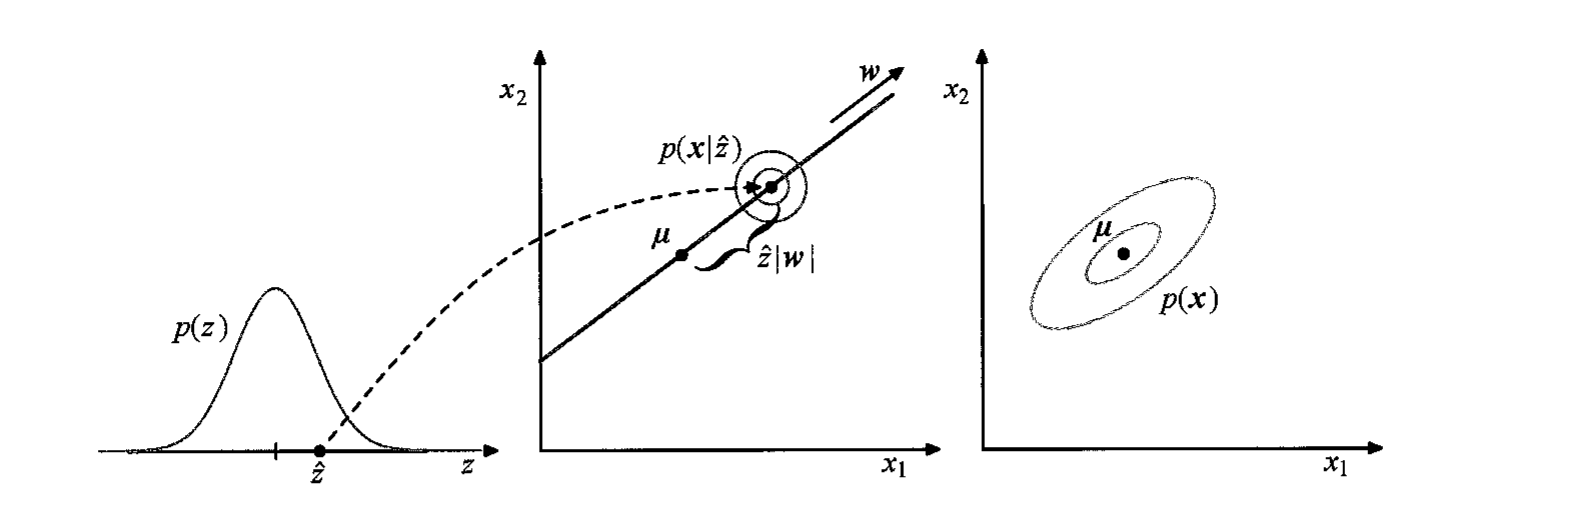
\includegraphics[width=0.95\textwidth]{ch16-fig16.7-ppca-generative.png}
  \caption{从常规 PCA 视角看一个针对两维数据空间和一维潜空间的概率 PCA 模型的生成过程。生成观测数据点 $\bm{x}$ 的过程是：首先从其先验分布 $p(\bm{z})$ 中抽取潜变量的一个值 $\hat{\bm{z}}$，然后从具有均值 $\bm{W}\hat{\bm{z}}+\bm{\mu}$ 和协方差 $\sigma^2\bm{I}$ 的各向同性 Gauss 分布（见红色圆圈）中抽取 $\bm{x}$ 的值。绿色椭圆显示了边缘分布 $p(\bm{x})$ 的密度等高线}
  \label{figure:ch16-PPCA生成过程}
\end{figure}

\subsection{似然函数}\label{subsection:ch16-似然函数}

假设我们希望通过最大似然法确定参数 $\bm{W}$、$\bm{\mu}$ 和 $\sigma^2$ 的值。为了写下似然函数，我们需要观测变量的边缘分布 $p(\bm{x})$ 的表达式。根据概率的加和法则与乘积法则，这可以表示为
\begin{align}
  p(\bm{x})=\int p(\bm{x}|\bm{z})p(\bm{z})\,\mathrm{d}\bm{z}.
  \label{align:ch16-边缘积分}
\end{align}

\begin{proposition}[概率 PCA 的边缘分布]\label{proposition:ch16-边缘分布}
在\cref{definition:ch16-概率PCA}的模型下，观测变量 $\bm{x}$ 的边缘分布仍是 Gauss 分布：
\begin{align}
  p(\bm{x})=\mathcal{N}(\bm{x}|\bm{\mu},\bm{C}),
  \label{align:ch16-边缘分布}
\end{align}
其中 $D\times D$ 的协方差矩阵 $\bm{C}$ 定义如下：
\begin{align}
  \bm{C}=\bm{W}\bm{W}^{\mathsf T}+\sigma^2\bm{I}.
  \label{align:ch16-边缘协方差}
\end{align}
\end{proposition}

\begin{proof}（重构新增）
把\eqref{align:ch16-条件分布}与\eqref{align:ch16-先验}代入\eqref{align:ch16-边缘积分}，并对指数配方。记 $\bm{M}=\bm{W}^{\mathsf T}\bm{W}+\sigma^2\bm{I}$，则被积函数为 $(2\pi\sigma^2)^{-D/2}(2\pi)^{-M/2}$ 乘以
\begin{align*}
  \exp\left\{-\frac{1}{2\sigma^2}\left\|\bm{x}-\bm{\mu}-\bm{W}\bm{z}\right\|^2-\frac{1}{2}\bm{z}^{\mathsf T}\bm{z}\right\}.
\end{align*}
把指数中 $\bm{z}$ 的二次型整理为
\begin{align*}
  -\frac{1}{2}\bm{z}^{\mathsf T}\left(\frac{\bm{W}^{\mathsf T}\bm{W}}{\sigma^2}+\bm{I}\right)\bm{z}+\frac{1}{\sigma^2}\bm{z}^{\mathsf T}\bm{W}^{\mathsf T}(\bm{x}-\bm{\mu})-\frac{1}{2\sigma^2}\left\|\bm{x}-\bm{\mu}\right\|^2
  =-\frac{1}{2\sigma^2}\bm{z}^{\mathsf T}\bm{M}\bm{z}+\frac{1}{\sigma^2}\bm{z}^{\mathsf T}\bm{W}^{\mathsf T}(\bm{x}-\bm{\mu})-\frac{1}{2\sigma^2}\left\|\bm{x}-\bm{\mu}\right\|^2,
\end{align*}
其中用到 $\bm{M}=\bm{W}^{\mathsf T}\bm{W}+\sigma^2\bm{I}=\sigma^2\left(\bm{W}^{\mathsf T}\bm{W}/\sigma^2+\bm{I}\right)$。对 $\bm{z}$ 用标准 Gauss 积分
\begin{align*}
  \int\exp\left\{-\frac{1}{2\sigma^2}\bm{z}^{\mathsf T}\bm{M}\bm{z}+\frac{1}{\sigma^2}\bm{z}^{\mathsf T}\bm{b}\right\}\mathrm{d}\bm{z}=(2\pi\sigma^2)^{M/2}|\bm{M}|^{-1/2}\exp\left\{\frac{1}{2\sigma^2}\bm{b}^{\mathsf T}\bm{M}^{-1}\bm{b}\right\},
\end{align*}
取 $\bm{b}=\bm{W}^{\mathsf T}(\bm{x}-\bm{\mu})$，得到 $p(\bm{x})$ 等于 $(2\pi)^{-D/2}(\sigma^2)^{-(D-M)/2}|\bm{M}|^{-1/2}$ 乘以
\begin{align*}
  \exp\left\{-\frac{1}{2\sigma^2}\left\|\bm{x}-\bm{\mu}\right\|^2+\frac{1}{2\sigma^2}(\bm{x}-\bm{\mu})^{\mathsf T}\bm{W}\bm{M}^{-1}\bm{W}^{\mathsf T}(\bm{x}-\bm{\mu})\right\}.
\end{align*}
再把指数写成单一二次型：
\begin{align*}
  -\frac{1}{2}(\bm{x}-\bm{\mu})^{\mathsf T}\left[\frac{1}{\sigma^2}\bm{I}-\frac{1}{\sigma^2}\bm{W}\bm{M}^{-1}\bm{W}^{\mathsf T}\right](\bm{x}-\bm{\mu}).
\end{align*}
方括号中的矩阵正是 $(\sigma^2\bm{I}+\bm{W}\bm{W}^{\mathsf T})^{-1}$：这可以由矩阵求逆恒等式\eqref{align:appA-求逆恒等式}取 $\bm{A}=\sigma^2\bm{I}$、$\bm{B}=\bm{W}$、$\bm{C}=\bm{I}$、$\bm{D}=\bm{W}^{\mathsf T}$ 得到，于是指数中的矩阵就是 $\bm{C}^{-1}$。最后核对归一化常数。由行列式恒等式，
\begin{align*}
  |\bm{C}|=\left|\sigma^2\bm{I}+\bm{W}\bm{W}^{\mathsf T}\right|=\sigma^{2D}\left|\bm{I}+\frac{\bm{W}^{\mathsf T}\bm{W}}{\sigma^2}\right|=\sigma^{2D}\cdot\sigma^{-2M}|\bm{M}|=\sigma^{2(D-M)}|\bm{M}|,
\end{align*}
故 $(\sigma^2)^{-(D-M)/2}|\bm{M}|^{-1/2}=|\bm{C}|^{-1/2}$，从而 $p(\bm{x})=(2\pi)^{-D/2}|\bm{C}|^{-1/2}\exp\{-\frac{1}{2}(\bm{x}-\bm{\mu})^{\mathsf T}\bm{C}^{-1}(\bm{x}-\bm{\mu})\}$，即\eqref{align:ch16-边缘分布}与\eqref{align:ch16-边缘协方差}。
\end{proof}

% SUPPLEMENT: parent=proposition:ch16-边缘分布; kind=motivation; location=紧随其后的 remark（重构新增）
\begin{remark}（重构新增）
这个命题说明：线性-Gauss 结构对边缘化是封闭的——把 Gauss 潜变量积掉之后仍然是 Gauss 分布，且协方差是“信号项”$\bm{W}\bm{W}^{\mathsf T}$ 与“噪声项”$\sigma^2\bm{I}$ 之和。这条可加性正是后面所有解释的基础。

条件的作用：$\sigma^2>0$ 保证 $\bm{C}$ 正定（$\bm{W}\bm{W}^{\mathsf T}$ 半正定，加上正定的 $\sigma^2\bm{I}$ 后严格正定），因此 $|\bm{C}|>0$、$\bm{C}^{-1}$ 存在，密度良定义；若允许 $\sigma^2=0$ 且 $M<D$，$\bm{C}$ 奇异，$p(\bm{x})$ 退化到子空间上。推导中唯二用到外部结果的地方是矩阵求逆恒等式与行列式恒等式，两者都在\hyperref[chapter:appA-线性代数]{附录\ref*{chapter:appA-线性代数}}中给出并证明，因此本证明不依赖本章后面的内容。
\end{remark}

注意预测分布也是 Gauss 分布，因此通过使用\eqref{align:ch16-生成过程}计算其均值和协方差就能更直接地得出同样的结果，于是有
\begin{align}
  \mathbb{E}[\bm{x}]=\mathbb{E}[\bm{W}\bm{z}+\bm{\mu}+\bm{\varepsilon}]=\bm{\mu},
  \label{align:ch16-边缘均值}
\end{align}
\begin{align}
  \operatorname{cov}[\bm{x}]&=\mathbb{E}\left[(\bm{W}\bm{z}+\bm{\varepsilon})(\bm{W}\bm{z}+\bm{\varepsilon})^{\mathsf T}\right]\nonumber\\
  &=\mathbb{E}\left[\bm{W}\bm{z}\bm{z}^{\mathsf T}\bm{W}^{\mathsf T}\right]+\mathbb{E}\left[\bm{\varepsilon}\bm{\varepsilon}^{\mathsf T}\right]\nonumber\\
  &=\bm{W}\bm{W}^{\mathsf T}+\sigma^2\bm{I},
  \label{align:ch16-边缘协方差推导}
\end{align}
这里我们利用了如下事实：$\bm{z}$ 和 $\bm{\varepsilon}$ 是独立随机变量，因此它们不相关。

直观上，我们可以认为分布 $p(\bm{x})$ 是通过取一个各向同性的 Gauss“喷雾罐”，然后在主成分子空间上移动并喷洒以 $\sigma^2$ 决定密度的Gauss墨水，并通过先验分布来加权的。累积的墨水密度将产生一个代表边缘密度 $p(\bm{x})$ 的“松饼”状分布。

\subsection{最大似然法}\label{subsection:ch16-最大似然法}

预测分布 $p(\bm{x})$ 受参数 $\bm{\mu}$、$\bm{W}$ 和 $\sigma^2$ 的控制。然而，这种参数化中存在冗余，相当于潜空间坐标发生旋转。为了说明这一点，考虑一个矩阵 $\widetilde{\bm{W}}=\bm{W}\bm{R}$，其中 $\bm{R}$ 是一个正交矩阵。利用正交性质 $\bm{R}\bm{R}^{\mathsf T}=\bm{I}$，我们看到出现在协方差矩阵 $\bm{C}$ 中的量 $\widetilde{\bm{W}}\widetilde{\bm{W}}^{\mathsf T}$ 具有以下形式：
\begin{align}
  \widetilde{\bm{W}}\widetilde{\bm{W}}^{\mathsf T}=\bm{W}\bm{R}\bm{R}^{\mathsf T}\bm{W}^{\mathsf T}=\bm{W}\bm{W}^{\mathsf T}.
  \label{align:ch16-旋转不变}
\end{align}

正因为独立于 $\bm{R}$，所以存在一整套矩阵 $\widetilde{\bm{W}}$，所有这些矩阵都会导致相同的预测分布。这种不变性可以理解为潜空间内的旋转。稍后我们将返回讨论该模型中独立参数的数量问题。

当计算预测分布时，我们需要 $\bm{C}^{-1}$，它涉及计算一个 $D\times D$ 矩阵的逆[参见\eqref{align:appA-求逆恒等式}]：
\begin{align}
  \bm{C}^{-1}=\sigma^{-2}\bm{I}-\sigma^{-2}\bm{W}\bm{M}^{-1}\bm{W}^{\mathsf T},
  \label{align:ch16-协方差逆}
\end{align}
其中 $M\times M$ 矩阵 $\bm{M}$ 定义如下：
\begin{align}
  \bm{M}=\bm{W}^{\mathsf T}\bm{W}+\sigma^2\bm{I}.
  \label{align:ch16-矩阵M}
\end{align}
因为我们求 $\bm{M}$ 的逆而不是直接求 $\bm{C}$ 的逆，所以计算 $\bm{C}^{-1}$ 的成本从 $\mathcal{O}(D^3)$ 降低到了 $\mathcal{O}(M^3)$。

除了预测分布 $p(\bm{x})$，我们还需要后验分布 $p(\bm{z}|\bm{x})$，后者可以直接再次使用线性-Gauss 模型的结果[\cref{proposition:ch03-线性GaussBayes}]写出：
\begin{align}
  p(\bm{z}|\bm{x})=\mathcal{N}\left(\bm{z}\left|\bm{M}^{-1}\bm{W}^{\mathsf T}(\bm{x}-\bm{\mu}),\sigma^2\bm{M}^{-1}\right.\right).
  \label{align:ch16-后验}
\end{align}

请注意，后验分布的均值依赖于 $\bm{x}$，而后验分布的协方差独立于 $\bm{x}$。

接下来考虑使用最大似然法确定模型参数。给定一组观测数据点的数据集 $\bm{X}=\{\bm{x}_n\}$，概率 PCA 模型可以表示为一个有向图，如\cref{figure:ch16-PPCA图模型}所示。相应的对数似然函数由\eqref{align:ch16-边缘分布}给出，形式为
\begin{align}
  \ln p(\bm{X}|\bm{\mu},\bm{W},\sigma^2)&=\sum_{n=1}^{N}\ln p(\bm{x}_n|\bm{W},\bm{\mu},\sigma^2)\nonumber\\
  &=-\frac{ND}{2}\ln(2\pi)-\frac{N}{2}\ln|\bm{C}|-\frac{1}{2}\sum_{n=1}^{N}(\bm{x}_n-\bm{\mu})^{\mathsf T}\bm{C}^{-1}(\bm{x}_n-\bm{\mu}).
  \label{align:ch16-对数似然}
\end{align}

\begin{figure}[htbp]
  \centering
  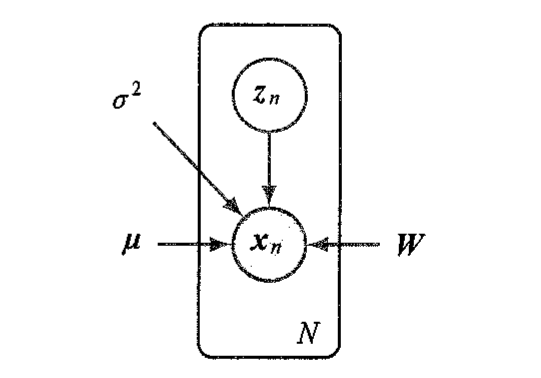
\includegraphics[width=0.30\textwidth]{ch16-fig16.8-ppca-graphical-model.png}
  \caption{对于包含 $\bm{x}$ 的 $N$ 次观测的一个数据集，概率 PCA 模型可以表示为一个有向图，其中的每个观测值 $\bm{x}_n$ 与潜变量的一个值 $\bm{z}_n$ 相关联}
  \label{figure:ch16-PPCA图模型}
\end{figure}

将对数似然函数关于 $\bm{\mu}$ 的导数设为零便可得到预期结果 $\bm{\mu}=\bar{\bm{x}}$，其中 $\bar{\bm{x}}$ 是由\eqref{align:ch16-均值}定义的数据均值。由于对数似然函数是 $\bm{\mu}$ 的二次函数，这个解代表了唯一的最大值，可以通过计算二阶导数来验证（见\cref{exercise:ch16-09}）。代入原式后，我们可以将对数似然函数写成以下形式：
\begin{align}
  \ln p(\bm{X}|\bm{W},\bm{\mu},\sigma^2)=-\frac{N}{2}\left\{D\ln(2\pi)+\ln|\bm{C}|+\operatorname{tr}\left(\bm{C}^{-1}\bm{S}\right)\right\},
  \label{align:ch16-对数似然约简}
\end{align}
其中 $\bm{S}$ 是由\eqref{align:ch16-协方差}定义的数据协方差矩阵。

虽然似然函数关于 $\bm{W}$ 和 $\sigma^2$ 的最大化更为复杂，但仍有精确的闭合解。Tipping and Bishop (1999) 指出，对数似然函数的所有驻点都可以写成
\begin{align}
  \bm{W}_{\text{ML}}=\bm{U}_M\left(\bm{L}_M-\sigma^2\bm{I}\right)^{1/2}\bm{R},
  \label{align:ch16-最大似然W}
\end{align}
其中 $\bm{U}_M$ 是一个 $D\times M$ 矩阵，其列由数据协方差矩阵 $\bm{S}$ 的任意子集（大小为 $M$）的特征向量给出。$M\times M$ 对角矩阵 $\bm{L}_M$ 的元素由对应的特征值 $\lambda_i$ 给出。$\bm{R}$ 是一个任意的 $M\times M$ 正交矩阵。

\begin{theorem}[概率 PCA 的最大似然解]\label{theorem:ch16-最大似然解}
设数据协方差矩阵 $\bm{S}$ 的特征值为 $\lambda_1\geqslant\cdots\geqslant\lambda_D>0$，对应的单位特征向量为 $\bm{u}_1,\cdots,\bm{u}_D$。对数似然函数\eqref{align:ch16-对数似然约简}关于 $\bm{W}$ 与 $\sigma^2$ 的所有驻点都由\eqref{align:ch16-最大似然W}与
\begin{align}
  \sigma^2_{\text{ML}}=\frac{1}{D-M}\sum_{i=M+1}^{D}\lambda_i
  \label{align:ch16-最大似然sigma}
\end{align}
给出，其中 $\bm{U}_M$、$\bm{L}_M$ 取 $\bm{S}$ 的一个大小为 $M$ 的特征向量子集及其特征值。当且仅当该子集是前 $M$ 个最大特征值时，该驻点使对数似然函数达到最大值；其余驻点（原文称为鞍点）的似然严格更小，都不是最大值点。
\end{theorem}

\begin{proof}（重构新增）
分三步。

第一步，关于 $\bm{W}$ 的驻点方程。由\eqref{align:ch16-对数似然约简}，并利用 $\partial\ln|\bm{C}|/\partial\bm{W}=2\bm{C}^{-1}\bm{W}$ 与 $\partial\operatorname{tr}(\bm{C}^{-1}\bm{S})/\partial\bm{W}=-2\bm{C}^{-1}\bm{S}\bm{C}^{-1}\bm{W}$（\cref{proposition:appA-矩阵导数恒等式}与\cref{proposition:appA-对数行列式的矩阵导数}），得
\begin{align*}
  \frac{\partial\ln p}{\partial\bm{W}}=-\frac{N}{2}\left(2\bm{C}^{-1}\bm{W}-2\bm{C}^{-1}\bm{S}\bm{C}^{-1}\bm{W}\right)=N\bm{C}^{-1}\left(\bm{S}\bm{C}^{-1}\bm{W}-\bm{W}\right),
\end{align*}
故驻点满足 $\bm{S}\bm{C}^{-1}\bm{W}=\bm{W}$。

第二步，验证\eqref{align:ch16-最大似然W}满足该方程。设 $\bm{S}\bm{U}_M=\bm{U}_M\bm{L}_M$，$\bm{U}_M^{\mathsf T}\bm{U}_M=\bm{I}$。由 $\bm{C}=\bm{U}_M(\bm{L}_M-\sigma^2\bm{I})\bm{U}_M^{\mathsf T}+\sigma^2\bm{I}$（其中用到 $\bm{W}\bm{W}^{\mathsf T}=\bm{U}_M(\bm{L}_M-\sigma^2\bm{I})\bm{U}_M^{\mathsf T}$）可知，对 $\bm{U}_M$ 的每一列有 $\bm{C}\bm{u}_i=\lambda_i\bm{u}_i$，而在 $\bm{U}_M$ 的正交补上 $\bm{C}$ 等于 $\sigma^2\bm{I}$。于是
\begin{align*}
  \bm{C}^{-1}\bm{W}=\bm{U}_M\bm{L}_M^{-1}\left(\bm{L}_M-\sigma^2\bm{I}\right)^{1/2}\bm{R},
\end{align*}
从而
\begin{align*}
  \bm{S}\bm{C}^{-1}\bm{W}=\bm{U}_M\bm{L}_M\bm{L}_M^{-1}\left(\bm{L}_M-\sigma^2\bm{I}\right)^{1/2}\bm{R}=\bm{U}_M\left(\bm{L}_M-\sigma^2\bm{I}\right)^{1/2}\bm{R}=\bm{W},
\end{align*}
即驻点方程成立。关于 $\bm{R}$ 的任意性见\cref{proposition:ch16-旋转不可识别}。

第三步，关于 $\sigma^2$ 的驻点方程与最大值的比较。由 $\partial\ln|\bm{C}|/\partial\sigma^2=\operatorname{tr}(\bm{C}^{-1})$ 与 $\partial\operatorname{tr}(\bm{C}^{-1}\bm{S})/\partial\sigma^2=-\operatorname{tr}(\bm{C}^{-2}\bm{S})$，驻点条件为 $\operatorname{tr}(\bm{C}^{-1})=\operatorname{tr}(\bm{C}^{-2}\bm{S})$。代入第二步的谱表示：$\operatorname{tr}(\bm{C}^{-1})=\sum_{i\in J}\lambda_i^{-1}+(D-M)/\sigma^2$ 而 $\operatorname{tr}(\bm{C}^{-2}\bm{S})=\sum_{i\in J}\lambda_i^{-1}+\sigma^{-4}\sum_{i\notin J}\lambda_i$，其中 $J$ 是所选取的特征向量下标集，$|J|=M$。两式相等给出 $(D-M)/\sigma^2=\sigma^{-4}\sum_{i\notin J}\lambda_i$，即 $\sigma^2=\frac{1}{D-M}\sum_{i\notin J}\lambda_i$，这正是\eqref{align:ch16-最大似然sigma}（当 $J$ 取前 $M$ 个下标时）。

把该 $\sigma^2$ 代回\eqref{align:ch16-对数似然约简}，并利用 $\operatorname{tr}(\bm{C}^{-1}\bm{S})=M+(D-M)=D$，得
\begin{align*}
  \ln p(\bm{X}|\bm{W},\bm{\mu},\sigma^2)=-\frac{N}{2}\left\{D\ln(2\pi)+\sum_{i\in J}\ln\lambda_i+(D-M)\ln\bar{\lambda}_{J^{\mathsf c}}+D\right\},
\end{align*}
其中 $\bar{\lambda}_{J^{\mathsf c}}=\frac{1}{D-M}\sum_{i\notin J}\lambda_i$ 是被丢弃特征值的平均值。于是最大化似然等价于最小化
\begin{align*}
  f(J)=\sum_{i\in J}\ln\lambda_i+(D-M)\ln\bar{\lambda}_{J^{\mathsf c}}.
\end{align*}
设 $a\in J$、$b\notin J$ 且 $\lambda_b>\lambda_a$，把 $J$ 换成 $J'=J\setminus\{a\}\cup\{b\}$。记 $S_c=\sum_{i\notin J}\lambda_i$、$r=\lambda_b-\lambda_a>0$，则 $S_c\geqslant\lambda_b$，于是
\begin{align*}
  f(J')-f(J)=\ln\frac{\lambda_b}{\lambda_a}+(D-M)\ln\left(1-\frac{r}{S_c}\right)
  \leqslant\ln\frac{\lambda_b}{\lambda_a}+(D-M)\ln\frac{\lambda_a}{\lambda_b}
  =\bigl(1-(D-M)\bigr)\ln\frac{\lambda_b}{\lambda_a}\leqslant0,
\end{align*}
其中第二个不等号用了 $r/S_c\leqslant r/\lambda_b=1-\lambda_a/\lambda_b$ 以及 $\ln$ 的单调性，最后一个不等号用了 $D-M\geqslant1$ 与 $\lambda_b>\lambda_a$。因此，只要保留的下标集合中存在比被丢弃的特征值更小的特征值，把它换成更大的那个就不会使似然变小；反复替换即知，最大值在 $J$ 取前 $M$ 个最大特征值时达到。若出现重特征值，则替换前后似然相同（最后一个不等号取等号），此时不同的 $J$ 给出相同的极大值，对应同一子空间，与命题中的“当且仅当”在子空间意义下一致。其余驻点的似然严格更小，不是最大值点。
\end{proof}

% SUPPLEMENT: parent=theorem:ch16-最大似然解; kind=motivation; location=紧随其后的 remark（重构新增）
\begin{remark}（重构新增）
本定理回答了“概率 PCA 到底在优化什么”这一问题：最大化似然自动把 $\bm{W}$ 的列对齐到样本协方差矩阵的前 $M$ 个特征向量，而 $\sigma^2$ 恰好等于被丢弃特征值的平均值。也就是说，概率模型的最大似然解在子空间层面就是\cref{section:ch16-主成分分析}中的主子空间，两种完全不同的出发点给出同一个答案；同时，$\sigma^2$ 给出了一个内生的噪声估计，这正是传统 PCA 所缺少的。

条件与边界需要说明。第一，要求所有 $\lambda_i>0$，否则 $\ln\lambda_i$ 无定义、$\bm{C}$ 奇异；当 $N<D$ 时会出现零特征值，此时应先用\cref{subsection:ch16-高维数据}的对偶技巧把问题降到 $N$ 维再应用本定理。第二，要求 $M\leqslant D-1$，否则\eqref{align:ch16-最大似然sigma}的分母为零；当 $M=D$ 时模型退化为无约束 Gauss 分布，见\eqref{align:ch16-满秩协方差}的讨论。第三，$\bm{R}$ 的任意性说明 $\bm{W}$ 本身不可辨识，可辨识的只是它张成的子空间与 $\sigma^2$；这一点由\cref{proposition:ch16-旋转不可识别}给出精确表述。最后，本证明第三步只用到 $\ln$ 的单调性与一个初等不等式，没有使用 EM 算法，因此不依赖\cref{subsection:ch16-EM算法}，不存在循环论证。
\end{remark}

此外，Tipping and Bishop (1999) 还指出，当选择那些对应于前 $M$ 个最大的特征值的特征向量时，就会得到似然函数的最大值（所有其他解都是鞍点）。Roweis (1998) 也独立提出了类似的猜想，尽管没有给出证明。同样，假设特征向量已按照对应特征值递减的顺序排列，则 $M$ 个主特征向量是 $\bm{u}_1,\cdots,\bm{u}_M$。在这种情况下，$\bm{W}$ 的列定义了标准 PCA 的主子空间。$\sigma^2_{\text{ML}}$ 是与被丢弃维度相关联的平均方差。

$\bm{R}$ 是正交的，因此可以解释为 $M$ 维潜空间中的旋转矩阵。如果我们将 $\bm{W}$ 的解代入 $\bm{C}$ 的表达式并利用正交性质 $\bm{R}\bm{R}^{\mathsf T}=\bm{I}$，就可以看到 $\bm{C}$ 独立于 $\bm{R}$。这表明预测密度不受潜空间内部旋转的影响。对于特殊情况 $\bm{R}=\bm{I}$，我们可以看到 $\bm{W}$ 的列是主成分特征向量，按方差参数 $\lambda_i-\sigma^2$ 缩放。一旦认识到独立 Gauss 分布（在这种情况下是潜空间分布和噪声模型）的卷积的方差是可加的，这些缩放因子的解释也就清楚了。因此，沿着特征向量 $\bm{u}_i$ 方向的方差 $\lambda_i$ 由以下两部分之和构成：一是单位方差潜空间分布通过 $\bm{W}$ 的对应列投影到数据空间的贡献 $\lambda_i-\sigma^2$，二是噪声模型在所有方向上添加的各向同性方差贡献 $\sigma^2$。

我们有必要花些时间研究\eqref{align:ch16-边缘协方差}给出的数据协方差矩阵的形式。考虑预测分布沿某个由单位向量 $\bm{v}$ 指定的方向的方差，其中 $\bm{v}^{\mathsf T}\bm{v}=1$，由 $\bm{v}^{\mathsf T}\bm{C}\bm{v}$ 给出。首先假设 $\bm{v}$ 与主子空间正交，换句话说，$\bm{v}$ 是由被丢弃特征向量的某种线性组合给出的。由于 $\bm{v}^{\mathsf T}\bm{U}_M=\bm{0}$，因此 $\bm{v}^{\mathsf T}\bm{C}\bm{v}=\sigma^2$。该模型预测了正交于主子空间的噪声方差。从\eqref{align:ch16-最大似然sigma}来看，它正是被丢弃特征值的平均值。假设 $\bm{v}=\bm{u}_i$，其中 $\bm{u}_i$ 是定义主子空间的保留特征向量之一，则有 $\bm{v}^{\mathsf T}\bm{C}\bm{v}=(\lambda_i-\sigma^2)+\sigma^2=\lambda_i$。

换句话说，这个模型正确地捕捉了数据沿主轴的方差，并用单个平均值 $\sigma^2$ 近似所有其余方向的方差。

\begin{proposition}[潜空间旋转的不可识别性]\label{proposition:ch16-旋转不可识别}
在概率 PCA 模型中，对任意 $M\times M$ 正交矩阵 $\bm{R}$，把 $\bm{W}$ 换成 $\bm{W}\bm{R}$、把 $\bm{z}$ 换成 $\bm{R}^{\mathsf T}\bm{z}$ 后，观测变量的边缘分布 $p(\bm{x})$ 与对数似然函数\eqref{align:ch16-对数似然约简}完全不变；因此仅由数据无法区分 $\bm{W}$ 与 $\bm{W}\bm{R}$。但 $\bm{W}$ 的列所张成的子空间与 $\sigma^2$ 是可以由数据唯一确定的（在特征值互不相同的条件下）。
\end{proposition}

\begin{proof}（重构新增）
由 $\bm{R}\bm{R}^{\mathsf T}=\bm{I}$ 得 $(\bm{W}\bm{R})(\bm{W}\bm{R})^{\mathsf T}=\bm{W}\bm{R}\bm{R}^{\mathsf T}\bm{W}^{\mathsf T}=\bm{W}\bm{W}^{\mathsf T}$，故 $\bm{C}$ 不变；由\eqref{align:ch16-边缘分布}，$p(\bm{x})$ 只通过 $\bm{C}$ 依赖于 $\bm{W}$，故边缘分布与似然函数都不变。另一方面，$p(\bm{z}|\bm{x})$ 的均值变为 $\bm{M}'^{-1}(\bm{W}\bm{R})^{\mathsf T}(\bm{x}-\bm{\mu})$，其中 $\bm{M}'=\bm{R}^{\mathsf T}\bm{M}\bm{R}$，即后验分布被 $\bm{R}^{\mathsf T}$ 旋转，这说明“潜变量本身”随 $\bm{R}$ 改变，不可由数据辨认。

反过来说，$\bm{C}=\bm{W}\bm{W}^{\mathsf T}+\sigma^2\bm{I}$ 的谱决定了一切：它的前 $M$ 个特征值是 $\lambda_1,\cdots,\lambda_M$、其余为 $\sigma^2$，特征向量给出主子空间。若 $\lambda_i$ 互不相同且与 $\sigma^2$ 不同，则这个谱分解唯一，于是主子空间与 $\sigma^2$ 被数据唯一确定，而 $\bm{W}$ 只被确定到右乘一个正交矩阵。这正是\eqref{align:ch16-最大似然W}中 $\bm{R}$ 的来源。
\end{proof}

% SUPPLEMENT: parent=proposition:ch16-旋转不可识别; kind=motivation; location=紧随其后的 remark（重构新增）
\begin{remark}（重构新增）
这条不可识别性与离散混合模型中“分量重标记”造成的不可识别性形成对照：那里的不可识别性是离散的（$K!$ 种重标记），这里的不可识别性是连续的（整个正交群 $O(M)$）。实践中的后果是：数值优化得到的 $\bm{W}$ 的列一般不正交，也不按特征值大小排列；若需要正交的主成分方向，可以对 $\bm{W}$ 作后处理（例如对 $\bm{W}\bm{W}^{\mathsf T}$ 作特征分解），或者修改 EM 算法使其直接产生按特征值排序的正交方向。

需要注意的是，不可识别的只是“坐标”，不是“模型”：所有 $\bm{W}\bm{R}$ 给出同一个预测密度，因此预测、似然、重构误差都不受影响。这也解释了为什么在概率 PCA 中谈“第 $k$ 个主成分”时必须先固定一个旋转约定（例如取 $\bm{R}=\bm{I}$ 并按特征值降序排列）。
\end{remark}

构建最大似然密度模型的一种方法是，简单地找到数据协方差矩阵的特征向量和特征值，然后使用上述结果计算 $\bm{W}$ 和 $\sigma^2$。在这种情况下，选择 $\bm{R}=\bm{I}$ 会更为方便。然而，如果我们通过数值优化似然函数来找到最大似然解，例如使用共轭梯度算法（Fletcher, 1987; Nocedal and Wright, 1999）或 EM 算法，那么得到的 $\bm{R}$ 矩阵的值本质上是任意的（见\cref{subsection:ch16-PCA的EM算法}）。这意味着矩阵 $\bm{W}$ 的列不必是正交的。如果需要正交基，则可以适当对 $\bm{W}$ 矩阵进行后处理（Golub and Van Loan, 1996）。也可以修改 EM 算法，以直接产生按相应特征值大小排序的正交主成分方向（Ahn and Oh, 2003）。

潜空间中的旋转不变性表示了一种统计上的不可识别性，类似于我们在离散潜变量混合模型中遇到的情况。这里，参数的连续性使得任何值都会导致相同的预测密度，这与混合设置中组件重标记相关的离散不可识别性形成了对比。

考虑 $M=D$，也就是没有降维的情况，则 $\bm{U}_M=\bm{U}$ 且 $\bm{L}_M=\bm{L}$。利用正交性质 $\bm{U}\bm{U}^{\mathsf T}=\bm{I}$ 和 $\bm{R}\bm{R}^{\mathsf T}=\bm{I}$，$\bm{x}$ 的边缘分布的数据协方差矩阵 $\bm{C}$ 将变为
\begin{align}
  \bm{C}&=\bm{U}\left(\bm{L}-\sigma^2\bm{I}\right)^{1/2}\bm{R}\bm{R}^{\mathsf T}\left(\bm{L}-\sigma^2\bm{I}\right)^{1/2}\bm{U}^{\mathsf T}+\sigma^2\bm{I}\nonumber\\
  &=\bm{U}\bm{L}\bm{U}^{\mathsf T}=\bm{S}.
  \label{align:ch16-满秩协方差}
\end{align}
于是我们得到无约束 Gauss 分布的标准最大似然解，其中数据协方差矩阵由样本协方差给出。

传统 PCA 通常构造为从 $D$ 维数据空间到 $M$ 维线性子空间的点的投影。然而，概率 PCA 可以最自然地表示为从潜空间到数据空间的映射。对于可视化和数据压缩等应用，我们可以使用 Bayes 定理反转这个映射。随后，数据空间中的任何点就可以由其在潜空间中的后验均值和协方差来概括。从\eqref{align:ch16-后验}可知，均值由下式给出：
\begin{align}
  \mathbb{E}[\bm{z}|\bm{x}]=\bm{M}^{-1}\bm{W}_{\text{ML}}^{\mathsf T}(\bm{x}-\bar{\bm{x}}),
  \label{align:ch16-后验均值}
\end{align}
其中 $\bm{M}$ 由\eqref{align:ch16-矩阵M}给出。这会将点投影到由下式给出的数据空间中：
\begin{align}
  \bm{W}\,\mathbb{E}[\bm{z}|\bm{x}]+\bm{\mu}.
  \label{align:ch16-重建映射}
\end{align}
请注意，这与正则化线性回归的方程相同，并且是最大化线性-Gauss 模型的似然函数的结果（见\cref{subsection:ch04-正则化最小二乘}）。同样，从\eqref{align:ch16-后验}可以看出，后验协方差由 $\sigma^2\bm{M}^{-1}$ 给出，且与 $\bm{x}$ 无关。

取极限 $\sigma^2\rightarrow0$，后验均值可以简化为
\begin{align}
  \left(\bm{W}_{\text{ML}}^{\mathsf T}\bm{W}_{\text{ML}}\right)^{-1}\bm{W}_{\text{ML}}^{\mathsf T}(\bm{x}-\bar{\bm{x}}).
  \label{align:ch16-投影极限}
\end{align}
这代表数据点在潜空间中的正交投影，因此我们恢复了标准 PCA 模型（见\cref{exercise:ch16-11}）。然而，在这个极限下，后验协方差为零，密度变得奇异。对于 $\sigma^2>0$，潜投影相对于正交投影向原点移动（见\cref{exercise:ch16-12}）。

最后请注意，概率 PCA 模型的一个重要作用是定义了一个多元 Gauss 分布，其中自由度的数量（也就是独立参数的数量）是可以控制的，同时仍允许模型捕获数据中的主要相关性。请回想一下，一个普通的 Gauss 分布在协方差矩阵中有 $D(D+1)/2$ 个独立参数（另外还有 $D$ 个参数在均值中）（见\cref{section:ch03-多元Gauss分布}）。因此，参数的数量随着 $D$ 的增加而按平方增长，并且在高维空间中可能会变得过多。如果我们限制协方差矩阵为对角矩阵，那便只有 $D$ 个独立参数，参数的数量随维度线性增长。然而，这会将变量当作独立变量，因此已无法再表达它们之间的任何相关性。概率 PCA 模型提供了一个优雅的折中方案，其中 $M$ 个最重要的相关性可以捕获，同时确保参数的数量只随维度线性增长。我们可以通过计算概率 PCA 模型中自由度的量看到这一点。数据协方差矩阵 $\bm{C}$ 取决于 $\bm{W}$，大小为 $D\times M$，再加上 $\sigma^2$，总共有 $DM+1$ 个参数。然而，我们已经看到这种参数化中存在与潜空间坐标系的旋转相关的一些冗余。表达这些旋转的正交矩阵 $\bm{R}$ 的大小为 $M\times M$。在这个矩阵的第一列中，有 $M-1$ 个独立参数（因为列向量必须归一化为单位长度）；而在第二列中，有 $M-2$ 个独立参数（因为列必须归一化并且与前一列正交），以此类推。将这个等差数列求和后，我们看到 $\bm{R}$ 总共有 $M(M-1)/2$ 个独立参数。因此，数据协方差矩阵 $\bm{C}$ 中自由度的数量由下式给出：
\begin{align}
  DM+1-M(M-1)/2.
  \label{align:ch16-参数计数}
\end{align}

在固定 $M$ 的情况下，该模型中独立参数的数量仅随维度线性增长。取 $M=D-1$，便可得到全协方差 Gauss 分布的标准结果（见\cref{exercise:ch16-14}）。在这种情况下，沿 $D-1$ 个线性无关方向的方差由 $\bm{W}$ 的列控制，而沿剩余方向的方差由 $\sigma^2$ 给出。当 $M=0$ 时，该模型等价于各向同性协方差的情况。

\subsection{因子分析}\label{subsection:ch16-因子分析}

因子分析模型是一个线性-Gauss 潜变量模型，它与概率 PCA 模型密切相关。因子分析的独特性体现为，其使得给定潜变量 $\bm{z}$ 的观测变量 $\bm{x}$ 的条件分布具有对角协方差，而不是各向同性协方差，即
\begin{align}
  p(\bm{x}|\bm{z})=\mathcal{N}(\bm{x}|\bm{W}\bm{z}+\bm{\mu},\bm{\Psi}),
  \label{align:ch16-因子条件}
\end{align}
其中 $\bm{\Psi}$ 是一个 $D\times D$ 的对角矩阵。

下面把上述模型的形式正式表述如下。

\begin{definition}[因子分析模型]\label{definition:ch16-因子分析}
设 $\bm{z}$ 是 $M$ 维潜变量，$\bm{x}$ 是 $D$ 维观测变量，且
\begin{align*}
  p(\bm{z})=\mathcal{N}(\bm{z}|\bm{0},\bm{I}),\qquad
  p(\bm{x}|\bm{z})=\mathcal{N}(\bm{x}|\bm{W}\bm{z}+\bm{\mu},\bm{\Psi}),
\end{align*}
其中 $\bm{W}$ 为 $D\times M$ 矩阵，$\bm{\Psi}$ 为 $D\times D$ 对角矩阵。则称 $(\bm{x},\bm{z})$ 服从因子分析（factor analysis）模型；称 $\bm{W}$ 的列为因子载荷（factor loading），称 $\bm{\Psi}$ 的对角元素为唯一性（uniquenesses）。
\end{definition}

% SUPPLEMENT: parent=definition:ch16-因子分析; kind=motivation; location=紧随其后的 remark（重构新增）
\begin{remark}（重构新增）
因子分析与概率 PCA 的唯一差别是条件协方差由 $\sigma^2\bm{I}$ 换成了对角矩阵 $\bm{\Psi}$。这一改动看似很小，却改变了模型能表达的相关结构：$\bm{W}\bm{W}^{\mathsf T}$ 负责解释变量之间的相关性，而 $\bm{\Psi}$ 的对角元 $\psi_i$ 单独描述第 $i$ 个变量自身的、无法由公共因子解释的方差。因此因子分析把每个观测变量的方差分解为“公共部分”$\sum_{j}w_{ij}^2$ 与“独特部分”$\psi_i$，这正是“因子载荷”“唯一性”这两个名称的含义。

条件方面：$\bm{\Psi}$ 必须正定（对角元全为正），否则条件密度退化；$\bm{W}$ 一般取满列秩 $M$，否则因子之间可以线性表示、模型进一步不可辨识。与概率 PCA 不同，这里不再有 $\sigma^2$ 这个共同的噪声水平，因此模型对潜空间的旋转不变，但对数据坐标的旋转不不变——这一点由\cref{exercise:ch16-17}精确刻画。正如本节将要说明的，$\bm{W}$ 没有闭式的最大似然解，需用 EM 或迭代方法求解。
\end{remark}

注意，因子分析模型和概率 PCA 模型一样，也假设观测变量 $x_1,\cdots,x_D$ 在给定潜变量 $\bm{z}$ 时是相互独立的。因子分析模型的核心在于，它通过用矩阵 $\bm{\Psi}$ 表示与每个坐标相关的独立方差，并在矩阵 $\bm{W}$ 中捕获变量之间的协方差，来解释观测到的数据协方差结构。

在 Everitt (1984)、Bartholomew (1987) 和 Basilevsky (1994) 等人的文献中可以找到关于因子分析的论述。Lawley (1953) 和 Anderson (1963) 研究了因子分析与 PCA 之间的联系，他们揭示了在似然函数的驻点处，对于一个 $\bm{\Psi}=\sigma^2\bm{I}$ 的因子分析模型，$\bm{W}$ 的列是样本协方差矩阵的缩放特征向量，而 $\sigma^2$ 是被丢弃特征值的平均值。后来，Tipping and Bishop (1999) 指出，在将组成 $\bm{W}$ 的特征向量选为主特征向量时，对数似然函数的最大值便会出现。

利用\eqref{align:ch16-边缘积分}，我们可以看到观测变量的边缘分布是由 $p(\bm{x})=\mathcal{N}(\bm{x}|\bm{\mu},\bm{C})$ 给出的，其中
\begin{align}
  \bm{C}=\bm{W}\bm{W}^{\mathsf T}+\bm{\Psi}.
  \label{align:ch16-因子协方差}
\end{align}

\begin{proposition}[因子分析的旋转不变性]\label{proposition:ch16-因子分析旋转不变}
对任意 $M\times M$ 正交矩阵 $\bm{R}$，把因子分析模型中的 $\bm{W}$ 换成 $\bm{W}\bm{R}$ 后，观测变量的边缘分布不变，即 $\bm{C}=\bm{W}\bm{W}^{\mathsf T}+\bm{\Psi}$ 不变；因此因子载荷矩阵 $\bm{W}$ 只能确定到右乘一个正交矩阵，因子本身（潜空间的坐标）不可识别。
\end{proposition}

\begin{proof}（重构新增）
$(\bm{W}\bm{R})(\bm{W}\bm{R})^{\mathsf T}=\bm{W}\bm{R}\bm{R}^{\mathsf T}\bm{W}^{\mathsf T}=\bm{W}\bm{W}^{\mathsf T}$，故\eqref{align:ch16-因子协方差}不变，从而 $p(\bm{x})$ 与似然函数不变。另一方面，给定 $\bm{x}$ 时 $\bm{z}$ 的后验均值是 $\bm{G}\bm{W}^{\mathsf T}\bm{\Psi}^{-1}(\bm{x}-\bm{\mu})$（其中 $\bm{G}$ 由\eqref{align:ch16-FA-G}定义），换成 $\bm{W}\bm{R}$ 后变为 $\bm{R}^{\mathsf T}$ 倍的相应量，即后验分布随 $\bm{R}$ 旋转，说明潜变量坐标确实改变。

反过来，模型能被数据确定的量是 $\bm{C}=\bm{W}\bm{W}^{\mathsf T}+\bm{\Psi}$。给定 $\bm{C}$ 与 $\bm{\Psi}$ 时 $\bm{W}\bm{W}^{\mathsf T}=\bm{C}-\bm{\Psi}$ 固定，而满足该式的 $\bm{W}$ 恰好构成 $\{\bm{W}\bm{R}:\bm{R}^{\mathsf T}\bm{R}=\bm{I}\}$ 这一族（因为 $\bm{W}$ 与 $\bm{W}\bm{R}$ 有相同的 Gram 矩阵，且同一 Gram 矩阵的满秩分解在右乘正交矩阵的意义下唯一）。故 $\bm{W}$ 的不可识别性恰为正交群 $O(M)$。
\end{proof}

% SUPPLEMENT: parent=proposition:ch16-因子分析旋转不变; kind=motivation; location=紧随其后的 remark（重构新增）
\begin{remark}（重构新增）
这条不可识别性比概率 PCA 的更“顽固”：在概率 PCA 中可以通过固定 $\bm{R}=\bm{I}$ 并按特征值大小排序来消除冗余（因为 $\sigma^2$ 提供了额外的标量约束），而在因子分析中，任意正交旋转都给出相同的似然，因此“第 $j$ 个因子是什么”没有数据依据。历史上人们曾试图通过旋转到某种“简单结构”（使载荷矩阵尽量稀疏）来解释各个因子，这种做法本质上是人为地添加了一个非统计的约定。

条件上要注意：该命题的结论依赖于 $\bm{\Psi}$ 固定且为对角。若允许同时变换 $\bm{\Psi}$，则群会变大，模型更加不可辨识（见\cref{exercise:ch16-17}的 (i) 款，那里对数据坐标作对角缩放会被 $\bm{\Psi}$ 吸收）。反之，若限定潜变量非 Gauss 分布，则旋转后的模型一般不再保持“各分量独立”，这正是独立成分分析能消除旋转不确定性的原因（见\cref{subsection:ch16-独立成分分析}）。
\end{remark}

与概率 PCA 模型一样，该模型对潜空间中的旋转是不变的（见\cref{exercise:ch16-16}）。

历史上，当人们尝试用因子分析方法对各个因子（$\bm{z}$ 空间中的坐标）进行解释时，曾引发争议。因子分析与这个空间中的旋转相关联，导致不可识别性，因而这种尝试被证明是有问题的。然而，从我们的角度看，我们将因子分析视为一种潜变量密度模型，关注的重点是其中潜空间的结构形式，而不是用于描述该空间的具体坐标。如果希望消除与潜空间旋转所带来的不确定性，则必须考虑非 Gauss 潜变量分布，以产生独立成分分析模型（参见\cref{subsection:ch16-独立成分分析}）。

概率 PCA 和因子分析的另一个区别是它们在数据集变换下的行为不同（见\cref{exercise:ch16-17}）。对于 PCA 和概率 PCA，如果旋转数据空间中的坐标系，则可以得到与数据完全相同的拟合结果，只不过 $\bm{W}$ 矩阵会由相应的旋转矩阵变换而成的。然而，对于因子分析，相似的性质是：如果我们对数据向量逐个分量地进行重新缩放，则这个操作会被吸收进相应的 $\bm{\Psi}$ 元素的重新缩放中。

\subsection{独立成分分析}\label{subsection:ch16-独立成分分析}

线性 Gauss 潜变量模型的一种扩展是这样的模型：观测变量与潜变量线性相关，但潜变量分布是非 Gauss 分布。这类模型的一个重要分支是独立成分分析（Independent Component Analysis, ICA）模型，其潜变量的联合分布能够分解为各分量的独立分布之积，即
\begin{align}
  p(\bm{z})=\prod_{j=1}^{M}p(z_j).
  \label{align:ch16-独立先验}
\end{align}

\begin{definition}[独立成分分析]\label{definition:ch16-独立成分分析}
设 $\bm{z}=(z_1,\cdots,z_M)$ 是潜变量，其联合分布满足\eqref{align:ch16-独立先验}（即各分量相互独立），且各分量 $z_j$ 的分布不是 Gauss 分布；观测变量由线性映射给出，$\bm{x}=\bm{W}\bm{z}+\bm{\mu}+\bm{\varepsilon}$，其中 $\bm{W}$ 为 $D\times M$ 矩阵、$\bm{\varepsilon}$ 为噪声。则称该模型为独立成分分析（Independent Component Analysis, ICA）模型。
\end{definition}

% SUPPLEMENT: parent=definition:ch16-独立成分分析; kind=motivation; location=紧随其后的 remark（重构新增）
\begin{remark}（重构新增）
ICA 要解决的问题是“盲源分离”：只观测到若干路混合信号，要求还原出彼此独立的原始源。与 PCA 相比，关键差别不在模型的形式（同样是线性映射），而在对潜变量的分布假设：PCA 默认潜变量是 Gauss 的，ICA 要求非 Gauss。

为什么非 Gauss 如此关键？因为 Gauss 分布在正交变换下保持 Gauss 且协方差为 $\bm{I}$ 的形式不变，所以只用二阶信息无法确定“哪个方向是源”；而非 Gauss 分布（尤其是重尾分布）在旋转下不再保持“各分量独立”这一性质，于是独立性本身成了可检验、可利用的约束。条件方面：$M\leqslant D$（通常取 $M=D$），$\bm{W}$ 需满列秩，否则源不可分离；噪声可省略是因为当 $M=D$ 且 $\bm{W}$ 非奇异时观测分布是源分布的确定性线性像，边缘分布通常非奇异。
\end{remark}

\begin{example}[ 盲源分离]\label{example:ch16-盲源分离}
为了理解这些模型的作用，可以设想以下场景：有两个人在同时说话，我们使用两个麦克风录制他们的声音。如果忽略时间延迟和回声等效果，则任何时刻麦克风接收到的信号都将由这两个声音的振幅的线性组合给出。这个线性组合的系数是恒定的。如果我们能从样本数据中推断出它们的值，我们就可以反转混合过程（假设它是非奇异的），从而得到两个干净的信号，每个信号只包含一个人的声音。这是一个盲源分离的问题，“盲”指的是我们只给出了混合数据，而没有观察到原始来源或混合系数（Cardoso, 1998）。
\end{example}

这类问题有时可以采取以下方法来解决（MacKay, 2003）。该方法忽略信号的时间特性，并将连续的样本视为独立同分布的。考虑一个生成式模型，其中有两个潜变量，对应于未观测语音信号振幅；还有两个观测变量，由麦克风处信号值给出。潜变量具有可以进行因子分解的联合分布，并且观测变量由潜变量的线性组合给出。没有必要包括噪声分布，因为潜变量的数量等于观测变量的数量，而观测变量的边缘分布通常不具有奇异性，所以观测变量仅仅是潜变量的确定性线性组合。给定一组观测数据，该模型的似然函数是线性组合中系数的一个函数。在使用基于梯度的优化方法最大化对数似然函数时，会产生特定版本的 ICA。

\begin{proposition}[Gauss 潜变量无法辨识独立成分]\label{proposition:ch16-Gauss不可辨识}
若把 ICA 模型中的潜变量分布换成一般的 Gauss 分布 $p(\bm{z})=\mathcal{N}(\bm{z}|\bm{m},\bm{\Sigma})$，则所得模型与某个概率 PCA 模型等价；特别地，对任意正交矩阵 $\bm{R}$，把 $\bm{z}$ 换成 $\bm{R}^{\mathsf T}\bm{z}$、$\bm{W}$ 换成 $\bm{W}\bm{R}$ 都给出同一个观测分布，而 $\bm{R}^{\mathsf T}\bm{z}$ 的各分量一般不再相互独立。因此仅凭二阶信息无法确定独立成分。
\end{proposition}

\begin{proof}（重构新增）
设 $\bm{\Sigma}=\bm{L}\bm{L}^{\mathsf T}$ 为 Cholesky 分解，令 $\bm{\xi}=\bm{L}^{-1}(\bm{z}-\bm{m})$，则 $\bm{\xi}\sim\mathcal{N}(\bm{0},\bm{I})$，且
\begin{align*}
  \bm{x}=\bm{W}\bm{z}+\bm{\mu}+\bm{\varepsilon}=\bm{W}\bm{L}\bm{\xi}+(\bm{W}\bm{m}+\bm{\mu})+\bm{\varepsilon}.
\end{align*}
这正是概率 PCA 模型\eqref{align:ch16-先验}—\eqref{align:ch16-条件分布}，参数为 $\bm{W}'=\bm{W}\bm{L}$、$\bm{\mu}'=\bm{W}\bm{m}+\bm{\mu}$。因此任何 Gauss 潜变量的线性模型都等价于一个概率 PCA 模型。

再由\cref{proposition:ch16-旋转不可识别}，对任意正交 $\bm{R}$，$(\bm{W}'\bm{R},\bm{R}^{\mathsf T}\bm{\xi})$ 与 $(\bm{W}',\bm{\xi})$ 给出相同的观测分布。把 $\bm{R}$ 取为一般的旋转，$\bm{R}^{\mathsf T}\bm{\xi}$ 的分量是独立标准正态变量的正交组合，仍是 Gauss 变量且彼此不相关；而 Gauss 情形下“不相关”与“独立”重合，因此任何正交组合都同时满足各分量独立，无法由数据判断哪一个坐标对应真正的源。若原模型中的源是非 Gauss 的独立分量，那么混入一个正交旋转后各分量不再独立（非 Gauss 情形下不相关推不出独立，见\cref{exercise:ch02-39}），正是这个差别使得 ICA 可解。
\end{proof}

% SUPPLEMENT: parent=proposition:ch16-Gauss不可辨识; kind=motivation; location=紧随其后的 remark（重构新增）
\begin{remark}（重构新增）
这条命题把“非 Gauss 性是 ICA 的必要条件”讲清楚了。直观上，Gauss 分布是唯一在正交变换下保持“独立同分布形式”的分布族：对 Gauss 变量而言，“不相关”与“独立”重合，因此旋转前后的两套坐标都满足独立假设，模型无法区分。非 Gauss 分布不具备这一旋转对称性，独立性才成为可用的判据。

条件上要注意：命题只说明 Gauss 情形不可辨识，并不说明任意非 Gauss 分布都可辨识。ICA 的可辨识性还需要至多一个源是 Gauss 的（否则仍可交换或旋转），以及混合矩阵满秩等条件；本书不展开这些充分条件，但读者应避免把“非 Gauss”误当成“一定可解”。
\end{remark}

对于为什么 Gauss 潜变量分布在线性模型中不足以找到独立成分，我们还可以用另一种方式来理解。我们注意到，主成分代表了数据空间中坐标系的旋转，目的是使协方差矩阵对角化，从而使新坐标中的数据分布不再相关。尽管零相关是独立性的必要条件，但它不是充分条件（见\cref{exercise:ch02-39}）。

在实践中，常用的潜变量分布由下式给出：
\begin{align}
  p(z_j)=\frac{1}{\pi\cos(z_j)}=\frac{2}{\pi\left(\mathrm{e}^{z_j}+\mathrm{e}^{-z_j}\right)}.
  \label{align:ch16-ICA密度}
\end{align}
与 Gauss 分布相比，它具有重尾（heavy tail），我们在许多真实世界的分布中也能观察到这种特性。

\begin{remark}（重构新增，原文问题说明）
\eqref{align:ch16-ICA密度}的第一个等号按字面并不成立：$\dfrac{1}{\pi\cos z_j}$ 在 $z_j=\pm\pi/2$ 处发散，且不是概率密度；而右端 $\dfrac{2}{\pi(\mathrm{e}^{z_j}+\mathrm{e}^{-z_j})}=\dfrac{1}{\pi\cosh z_j}$ 才是有定义、可归一化的重尾密度。原文此处印作 $\cos$，应为双曲余弦 $\cosh$ 的排印脱漏。本式保留原样以便与原文对照，但读者应按 $\cosh$ 理解：该密度确实具有比 Gauss 分布更重的尾部，这正是 ICA 所需要的性质。
\end{remark}

最初的 ICA 模型（Bell and Sejnowski, 1995）是采用信息最大化定义的目标函数进行优化。概率潜变量表述的一个优势是，它有助于启发并构建 ICA 的扩展。例如，独立因子分析（independent factor analysis）（Attias, 1999）考虑了一个模型，在该模型中，潜变量和观测变量的数量可以不同，观测变量是有噪声的，潜变量则具有 Gauss 混合模型化的灵活分布。可以使用 EM 算法最大化这个模型的对数似然函数，并使用变分法近似重构潜变量。研究人员考虑了许多其他类型的模型，如关于独立成分分析及其应用的文献已经不胜枚举了（Jutten and Herault, 1991; Comon, Jutten, and Herault, 1991; Amari, Cichocki, and Yang, 1996; Pearlmutter and Parra, 1997; Hyv\"arinen and Oja, 1997; Hinton et al., 2001; Miskin and MacKay, 2001; Hojen-Sorensen, Winther, and Hansen, 2002; Choudrey and Roberts, 2003; Chan, Lee, and Sejnowski, 2003; Stone, 2004）。

\subsection{Kalman 滤波器}\label{subsection:ch16-Kalman滤波器}

到目前为止，我们假设数据值是独立同分布的。一种常见的非独立同分布情况是，数据点形成一个有序序列。我们已经看到，隐 Markov 模型可以视为混合模型的扩展，旨在允许数据中存在序列相关性（参见\cref{subsection:ch15-Gauss混合em}）。类似地，连续潜变量模型可以通过连接潜变量形成 Markov 链来扩展，以处理序列数据，参见\cref{figure:ch16-Kalman图模型}所示的图模型。这种模型称为线性动态系统（linear dynamical system）或 Kalman 滤波器（Zarchan and Musoff, 2005）。注意，这与隐 Markov 模型的图结构相同（参见\cref{subsection:ch15-Gauss混合em}）。值得注意的是，隐 Markov 模型和线性动态系统是独立发展的。然而，一旦它们都表示为图模型，它们之间的深层关系就会水落石出。Kalman 滤波器已广泛地应用在许多实时跟踪应用中，如使用雷达信号跟踪飞机。

\begin{definition}[线性动态系统]\label{definition:ch16-线性动态系统}
设观测序列 $\bm{x}_1,\cdots,\bm{x}_N$ 与潜变量序列 $\bm{z}_1,\cdots,\bm{z}_N$ 满足：(i) 给定 $\bm{z}_n$ 时 $\bm{x}_n$ 的条件分布是线性-Gauss 模型 $p(\bm{x}_n|\bm{z}_n)$，其均值是 $\bm{z}_n$ 的线性函数、协方差与 $\bm{z}_n$ 无关；(ii) 潜变量构成 Markov 链，$p(\bm{z}_n|\bm{z}_{n-1})$ 是 Gauss 分布且其均值是 $\bm{z}_{n-1}$ 的线性函数；(iii) 所有 $p(\bm{x}_n|\bm{z}_n)$ 共享同一组参数，所有 $p(\bm{z}_n|\bm{z}_{n-1})$ 也共享同一组参数。则称该模型为线性动态系统（linear dynamical system），也称 Kalman 滤波器。
\end{definition}

% SUPPLEMENT: parent=definition:ch16-线性动态系统; kind=motivation; location=紧随其后的 remark（重构新增）
\begin{remark}（重构新增）
线性动态系统把概率 PCA 从“独立同分布样本”推广到“有序序列”：每个观测仍然由各自的潜变量经线性-Gauss 映射生成，但潜变量之间用 Markov 链串起来，从而让相邻时刻的状态可以相互传递信息。第 (iii) 条“参数共享”是关键：它使模型的参数个数与序列长度 $N$ 无关，因此无论序列多长，都只有固定个数的参数需要估计，这也是 Kalman 滤波可以实时运行的根本原因。

条件方面：$p(\bm{z}_n|\bm{z}_{n-1})$ 取线性-Gauss 形式保证了整个模型是线性-Gauss 的，从而所有边缘与条件分布都是 Gauss 分布；否则后验将不再有闭式，只能退化为一般的状态空间模型。若把 $p(\bm{x}_n|\bm{z}_n)$ 换成离散分布、$p(\bm{z}_n|\bm{z}_{n-1})$ 换成离散转移，就得到隐 Markov 模型——两者的图结构相同，差别只在变量的取值域。
\end{remark}

\begin{figure}[htbp]
  \centering
  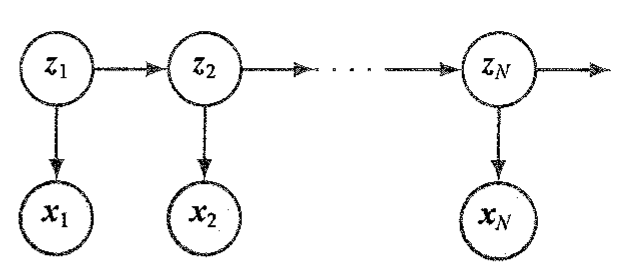
\includegraphics[width=0.62\textwidth]{ch16-fig16.9-kalman-graphical-model.png}
  \caption{用于序列数据的概率图模型称为线性动态系统或 Kalman 滤波器，其中的潜变量形成了一个 Markov 链}
  \label{figure:ch16-Kalman图模型}
\end{figure}

在这样的最简单模型中，\cref{figure:ch16-Kalman图模型}中的分布 $p(\bm{x}_n|\bm{z}_n)$ 代表了该特定观测结果的线性-Gauss 潜变量模型，就像我们之前讨论的独立同分布数据一样。然而，潜变量 $\bm{z}_n$ 不再视为独立的，而是形成了一个 Markov 链，链中每个潜变量的分布 $p(\bm{z}_n|\bm{z}_{n-1})$ 取决于链中前一个潜变量的状态。在线性-Gauss 潜变量模型中，$\bm{z}_n$ 的分布是 Gauss 分布，均值则由 $\bm{z}_{n-1}$ 的线性函数给出。通常，分布 $p(\bm{x}_n|\bm{z}_n)$ 的所有参数是共享的，分布 $p(\bm{z}_n|\bm{z}_{n-1})$ 的所有参数也是共享的，因此模型中总的参数数量是固定的，不依赖于序列的长度。这些参数可以通过最大似然法从数据中来学习。这需要用到在图模型上传播消息的有效算法（Bishop, 2006）。在本章的其余部分，我们将专注于独立同分布数据。

\end{document}
